\chapter{Verification and Validation}
\label{ch:vandv}
Simulations are a useful, efficient and cost-effective way to obtain insight into complex problems, such as the one described in this report. However, care must be taken to ensure that the simulation is free of errors, and that it provides an accurate representation of reality. This process is referred to as verification and validation. \\

As described earlier, verification through unit and integration testing was performed throughout the implementation process. As can be seen in the implementation \href{https://github.com/ArjanVermeulen97/thesis-code.git}{on Github}, the code is structured into smaller unit functions, such as rotation matrices, angle calculation functions, and fundamental equations such as Planck's law. These unit functions are integrated into more complex functions, such as reference frame transformations. This approach allows for manual testing of the software from the beginning of programming to ensure correctness of the simulation. In addition, throughout the process, several sources from literature were implemented. As these sources often do not provide details as to how to implement their findings, the resulting implementation should be checked against the data in the sources. This is especially important in the case of numerical integration schemes, where accuracy can be dependent on implementation. Therefore, further verification of the thermal infrared target and background signal is presented in \autoref{sec:vvinfrared}, and the algorithm for solving the orbital positions in \autoref{sec:vvsurvey}.\\

Verification of the software units and their implementation, however, is not enough to provide acceptable results. It also has to be shown that the simulation accurately portrays the problem being studied. In particular, the effect of major assumptions, as well as the results of the system for various test cases, should be examined. To this end, the possibly impactful assumption regarding survey cadence (as discussed in \autoref{sec:methodologyimplementation}) is checked. Finally, the results of the simulation tool are compared to the results of a previously validated simulation tool - the tool developed by \cite{2017NEOSDT} - to determine whether the results presented are an accurate representation of reality. This analysis is presented in \autoref{sec:vvperformance}.

\section{Infrared Signal}
\label{sec:vvinfrared}

\begin{figure}[htbp]
 \centering
 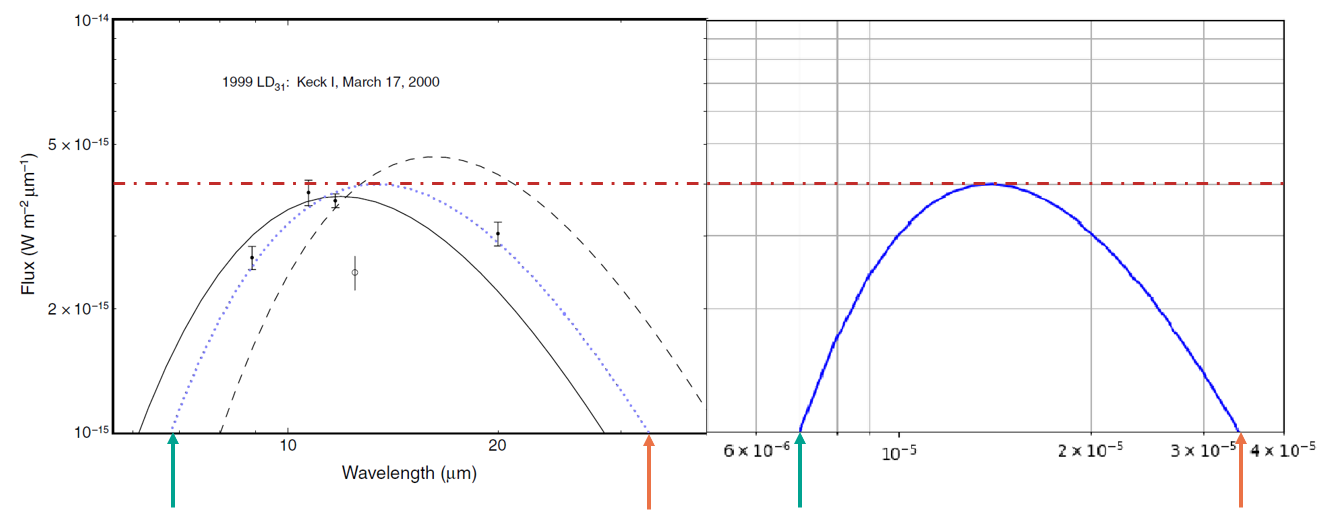
\includegraphics[width=0.7\textwidth]{img/validation_tir_target_signal.png}
 \caption{Comparison of infrared signal calculation. Reference data is shown on the left, obtained from \cite{AsteroidNEATM}. The other two curves in the plot were results of other, older, asteroid thermal models.}
 \label{fig:validation_tir_target_signal}
\end{figure}

For verification of the thermal infrared target signal, \cite{AsteroidNEATM} provide flux calculations for the asteroid 1999 LD$_{31}$, on a given date. Implementation of the thermal model was verified by repeating this simulation, and comparing the results. This comparison can be seen in \autoref{fig:validation_tir_target_signal}. Ephemeris was obtained \href{https://ssd.jpl.nasa.gov/tools/sbdb\_lookup.html#/?sstr=1999\%20LD31}{from NASA/JPL Small-Body Database}. The implementation provides the correct general shape of the curve, as well as correct maximum value and axis intercepts. Therefore it was concluded that the implementation is correct.\\

\begin{figure}[ph]
 \centering
 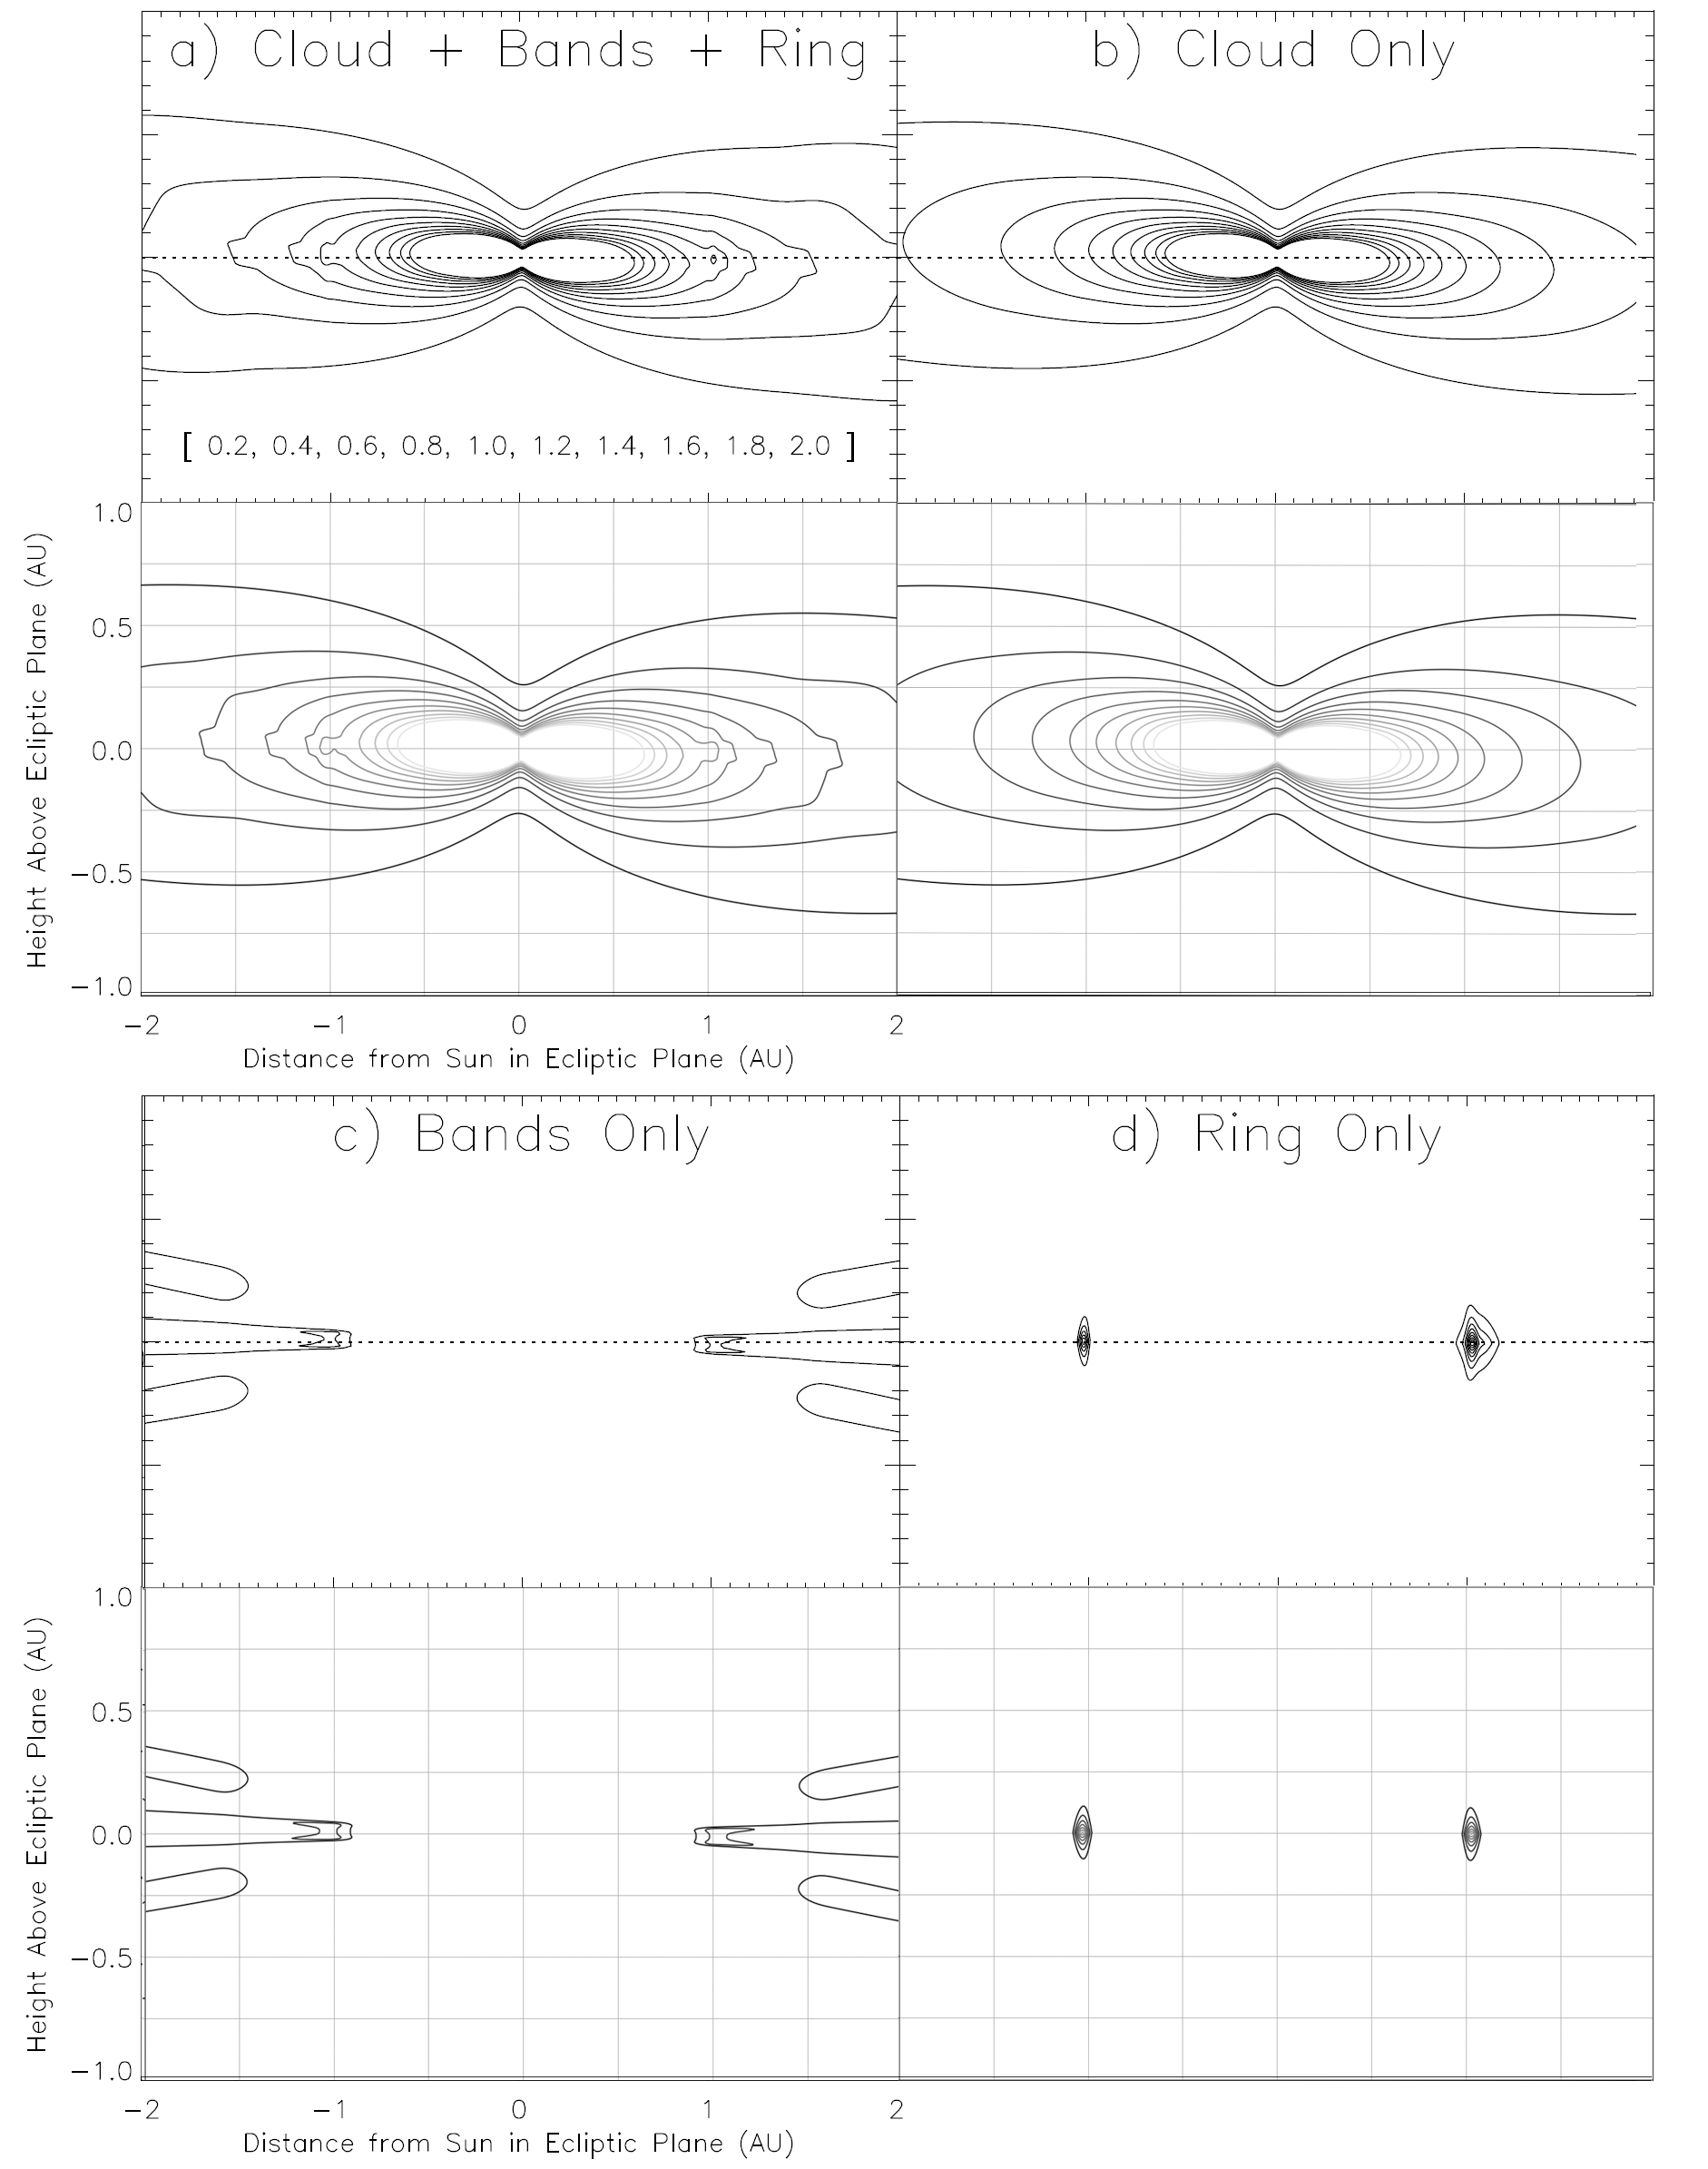
\includegraphics[width=1.0\textwidth]{img/validation_tir_background_signal.png}
 \caption{Comparison of the calculated densities of the various interplanetary dust components. Top: reference images from \cite{IRDust}, bottom: calculated densities.}
 \label{fig:validation_tir_background_signal}
\end{figure}

The second component of the infrared signal to be verified is the implementation of the interplanetary dust model provided by \cite{IRDust}. This process was conducted in two steps. Firstly, the calculated density models involve several complicated formulae, and are therefore subject to error. These were compared to implementation by \cite{IRDust} in \autoref{fig:validation_tir_background_signal}. It can be seen that the implementation matches the results of the authors. \\

\begin{table}[htbp]
\centering
\caption{Comparison of computed and reference values for the infrared zodiac light signal at $4.9\mu$m. Reference values according to \cite{IRDust}}
\label{tab:49irbackground}
\begin{tabular}{lll|l|lll}
($\lambda$, $\beta$)    & Date     & $\lambda_{\odot}$  & Component & Reference & Computed & Difference \\ \hline
122, 0  & 19-04-90 & 208.81 & Cloud     & 0.679     & 0.655    & -3.53\%    \\
        &          &        & Bands     & 0.0141    & 0.0121   & -14.2\%    \\
        &          &        & Ring      & 0.0164    & 0.0493   & 201\%      \\ \hline
        &          &        & Total     & 0.808     & 0.716    & -11.4\%    \\ \hline
137, 46 & 09-05-90 & 228.25 & Cloud     & 0.449     & 0.492    & 9.58\%     \\
        &          &        & Bands     & 0.0014    & 0.00102  & -27.1\%    \\
        &          &        & Ring      & 0.0251    & 0.00871  & -65.3\%    \\ \hline
        &          &        & Total     & 0.476     & 0.501    & 5.25\%    
\end{tabular}
\end{table}

\begin{table}[htbp]
\centering
\caption{Comparison of computed and reference values for the infrared zodiac light signal at $12\mu$m. Reference values according to \cite{IRDust}}
\label{tab:12irbackground}
\begin{tabular}{lll|l|lll}
($\lambda$, $\beta$)    & Date     & $\lambda_{\odot}$  & Component & Reference & Computed & Difference \\ \hline
122, 0  & 19-04-90 & 208.81 & Cloud     & 28.476    & 29.63    & 4.05\%     \\
        &          &        & Bands     & 1.938     & 1.78     & -8.15\%    \\
        &          &        & Ring      & 3.324     & 1.6      & -51.9\%    \\ \hline
        &          &        & Total     & 33.875    & 33.011   & -2.55\%    \\ \hline
137, 46 & 09-05-90 & 228.25 & Cloud     & 14.669    & 17.208   & 17.3\%     \\
        &          &        & Bands     & 0.0924    & 0.0868   & -6.06\%    \\
        &          &        & Ring      & 0.735     & 0.266    & -63.8\%    \\ \hline
        &          &        & Total     & 15.483    & 17.561   & 13.4\%    
\end{tabular}
\end{table}

The second step is required for judging the accuracy of the various numerical integrations involved in the model. This was done using reference values provided by the authors. The calculated and reference contributions for the various components in the two test cases can be seen in \autoref{tab:49irbackground} for the $4.9 \mu\mathrm{m}$ wavelength and \autoref{tab:12irbackground} for the $12 \mu\mathrm{m}$ background. Ephemerides were obtained \href{https://ssd.jpl.nasa.gov/horizons/}{from NASA/JPL Horizons System}. It can be seen in the tables that the error of the implementation is in the order of 10\%, which was deemed acceptable, given the nature of numerical integration of complicated functions. A point of note, however, is the large discrepancy in calculated values for the contribution of the circumsolar ring. This discrepancy is due to the fact that \cite{IRDust} include a contribution for an Earth-trailing blob of dust in their analysis. In the implementation presented here, this blob was omitted, as implementation of an addition Earth empheris would complicate the analysis, and impact was judged as small as the topic of interest is not - unlike the work of \cite{IRDust} - observation from Earth.

\section{Survey Implementation}
\label{sec:vvsurvey}
The second subject of additional inspection is the implementation of the survey components. Firstly, the implementation of the orbital mechanics and reference frame transformations has to be verified. In \autoref{fig:validation_theta_solve}, the modelled relationship between true anomaly and mean anomaly as a function of eccentricity is shown. The results of this are as expected (see e.g. \cite{Curtis}), meaning the algorithm for numerical approximation was implemented correctly, and works as predicted. Some cases, specifically for $e$ close to 1 and mean anomaly very close to $2\pi$ resulted in an initial guess of $\theta > 2\pi$ before differential corrections. This introduced an error in the code. For these cases it was found that setting $\theta = 2\pi$ provided a good solution. \\

\begin{figure}[htbp]
 \centering
 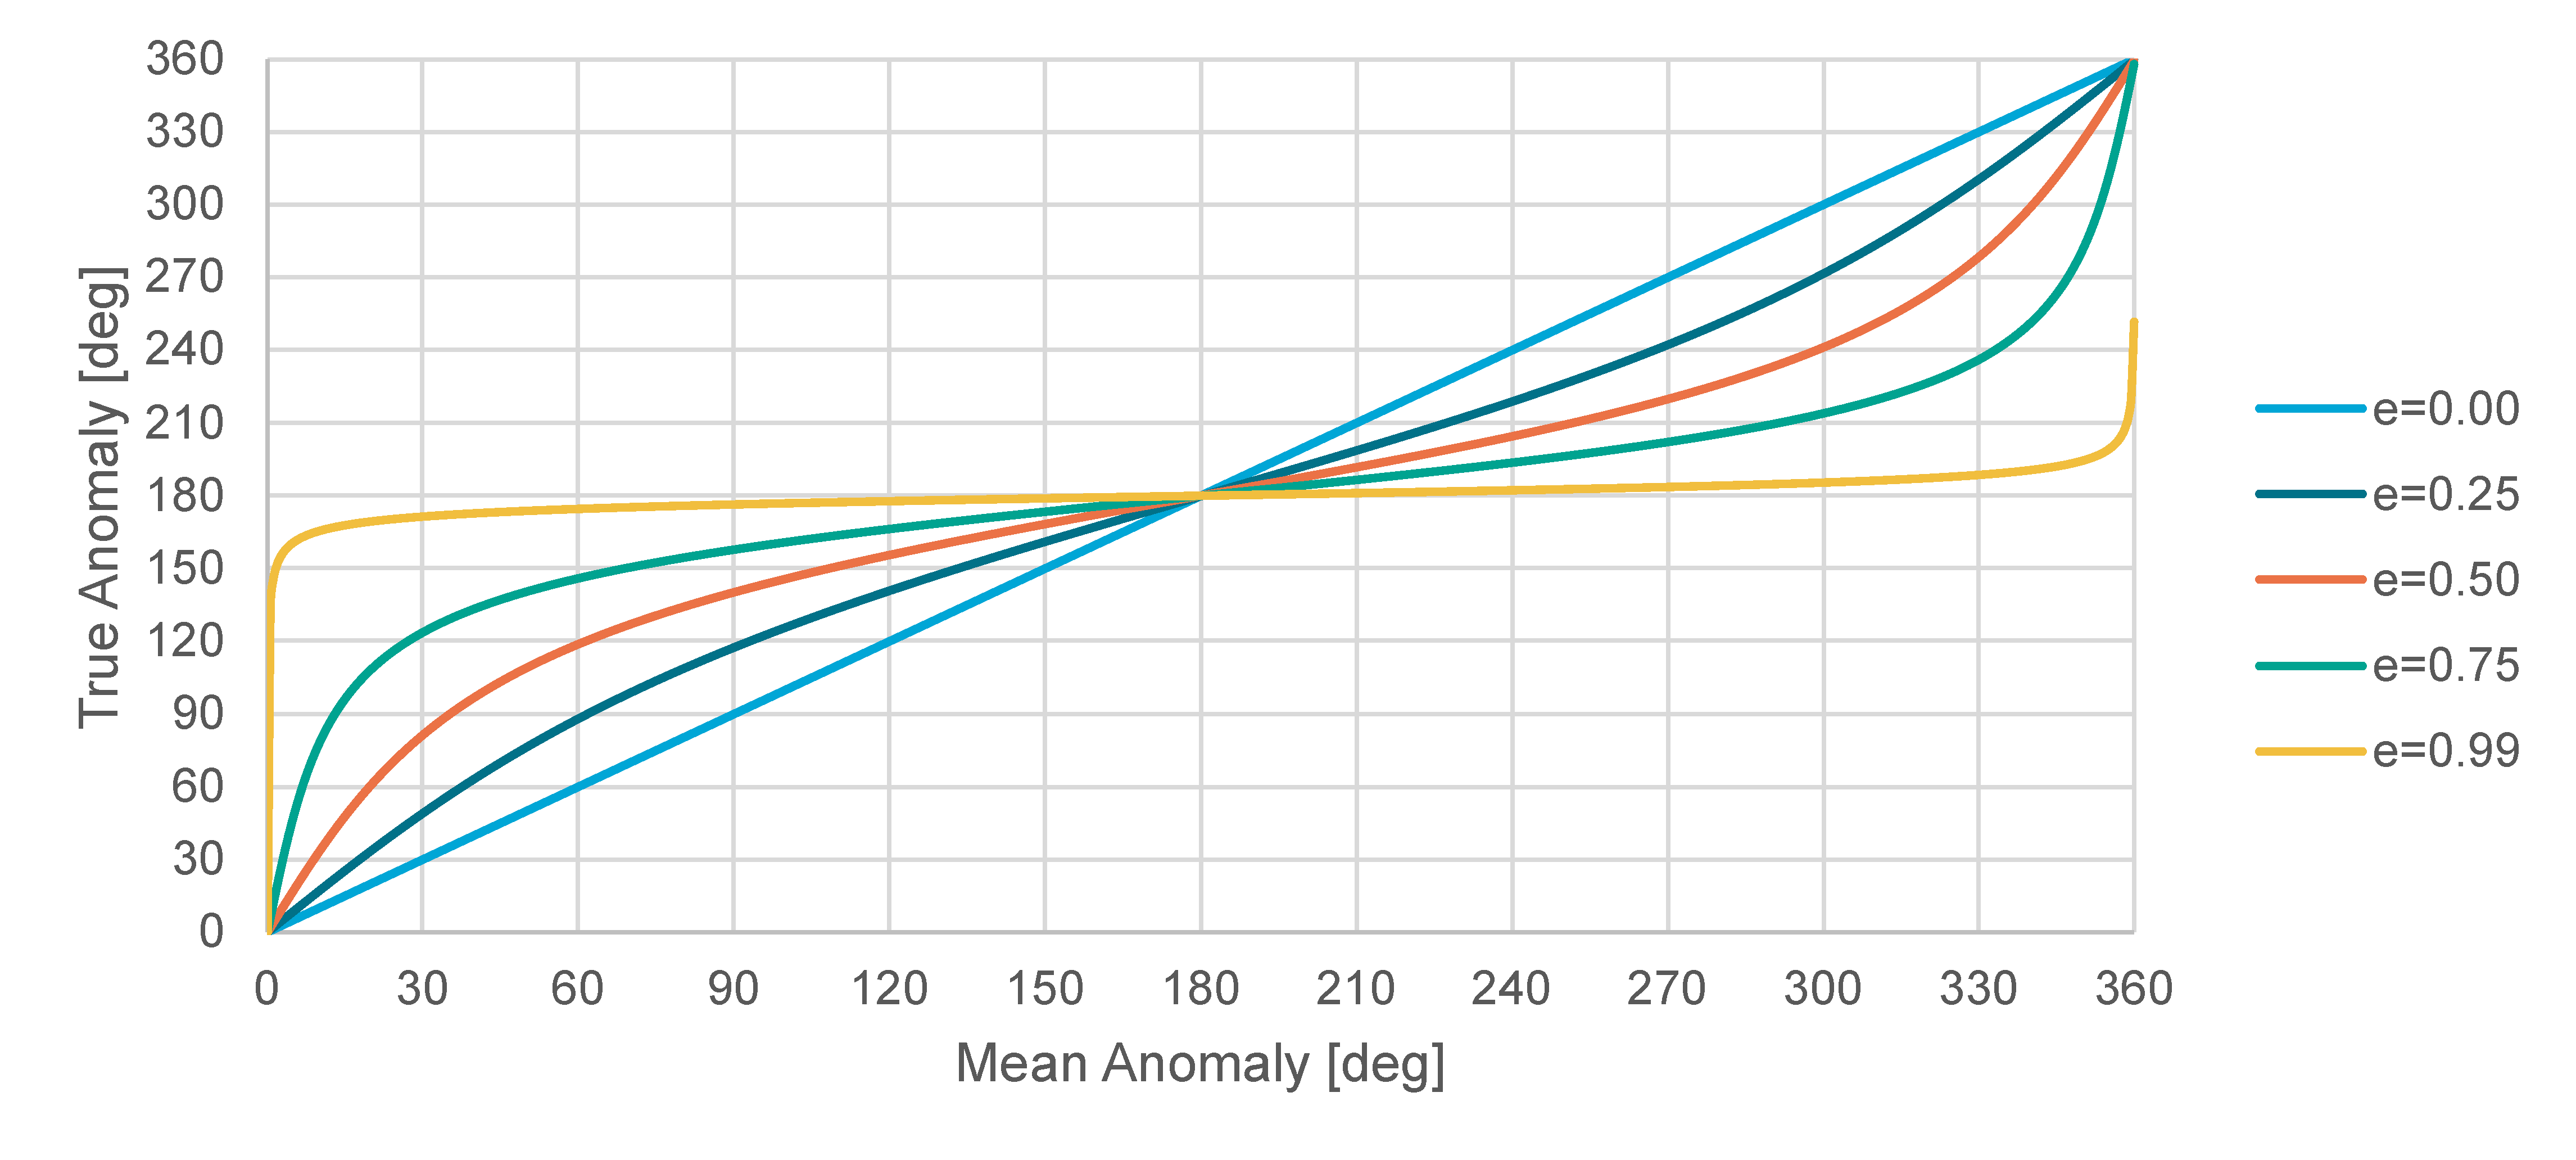
\includegraphics[width=0.7\textwidth]{img/validation_theta_solve.pdf}
 \caption{Relationship between mean anomaly and true anomaly for various eccentricities.}
 \label{fig:validation_theta_solve}
\end{figure}

The second part of the orbital propagation to be verified is the transformation from Keplerian orbital elements to cartesian coordinates. Reference frame transformations are infamously susceptible to error, and therefore a large set of reference calculations were performed for various combinations of orbital elements. A small, arbitrary, sample of these results is shown in \autoref{tab:keplertocartesian}. Distances are given in AU, angles in degrees. The transformations can be seen to be correct.\\

\begin{table}[htbp]
\centering
\caption{Comparison of computed and reference transformations from Keplerian orbital elements to cartesian coordinates.}
\label{tab:keplertocartesian}
\begin{tabular}{llllll|lll|lll}
$a$   & $e$   & $i$  & $\Omega$ & $\omega$ & $\theta$ & $x_c$      & $y_c$      & $z_c$     & $x_r$  & $y_r$  & $z_r$ \\ \hline
0.5 & 0   & 0  & 0    & 0       & 0     & 0.500  & 0.000  & 0.000 & 0.500  & 0.000  & 0.000 \\
0.5 & 0   & 90 & 180  & 90      & 90    & 0.500  & 0.000  & 0.000 & 0.500  & 0.000  & 0.000 \\
0.5 & 0.5 & 90 & 90   & 180     & 0     & 0.000  & -0.250 & 0.000 & 0.000  & -0.250 & 0.000 \\
0.5 & 0.9 & 45 & 90   & 0       & 180   & 0.000  & -0.950 & 0.000 & 0.000  & -0.950 & 0.000 \\
1   & 0   & 45 & 0    & 90      & 90    & -1.000 & 0.000  & 0.000 & -1.000 & 0.000  & 0.000 \\
1   & 0.5 & 0  & 180  & 180     & 180   & -1.500 & 0.000  & 0.000 & -1.500 & 0.000  & 0.000 \\
1   & 0.9 & 0  & 180  & 0       & 90    & 0.000  & -0.190 & 0.000 & 0.000  & -0.190 & 0.000 \\
2   & 0   & 0  & 90   & 90      & 0     & -2.000 & 0.000  & 0.000 & -2.000 & 0.000  & 0.000 \\
2   & 0   & 90 & 0    & 180     & 180   & 2.000  & 0.000  & 0.000 & 2.000  & 0.000  & 0.000 \\
2   & 0.5 & 90 & 0    & 0       & 90    & 0.000  & 0.000  & 1.500 & 0.000  & 0.000  & 1.500
\end{tabular}
\end{table}

Next, the assumption on the survey cadence will be validated. As discussed in \autoref{sec:methodologyimplementation}, this assumption was made to vastly decrease computational load, allowing numerical optimization through repeated simulations. Validation was performed through explicitly modelling the survey cadence as it would occur in reality for a range of spacecraft parameters (numerically optimizing the solutions was deemed infeasible due to the long computational time of these simulations), and comparing these to outputs of the simulation with the assumption applied. The resulting performances along with their standard deviation, is shown in \autoref{fig:validation_cadence_performance}. The error introduced by the assumption is minor, and it still accurately portrays the problem to be simulation. In fact, inspection of the difference between the simulations, shown in \autoref{fig:validation_cadence_error}, reveals the error to be in the order of 1-2\%. However, as is also shown in that figure, the variance in the results is far greater than the influence of this assumption. It is however concluded that the assumptions results in an approximate 1\% underestimation of the performance of the system, which was deemed acceptable for the benefits provided by the assumption.

\begin{figure}[htbp]
 \centering
 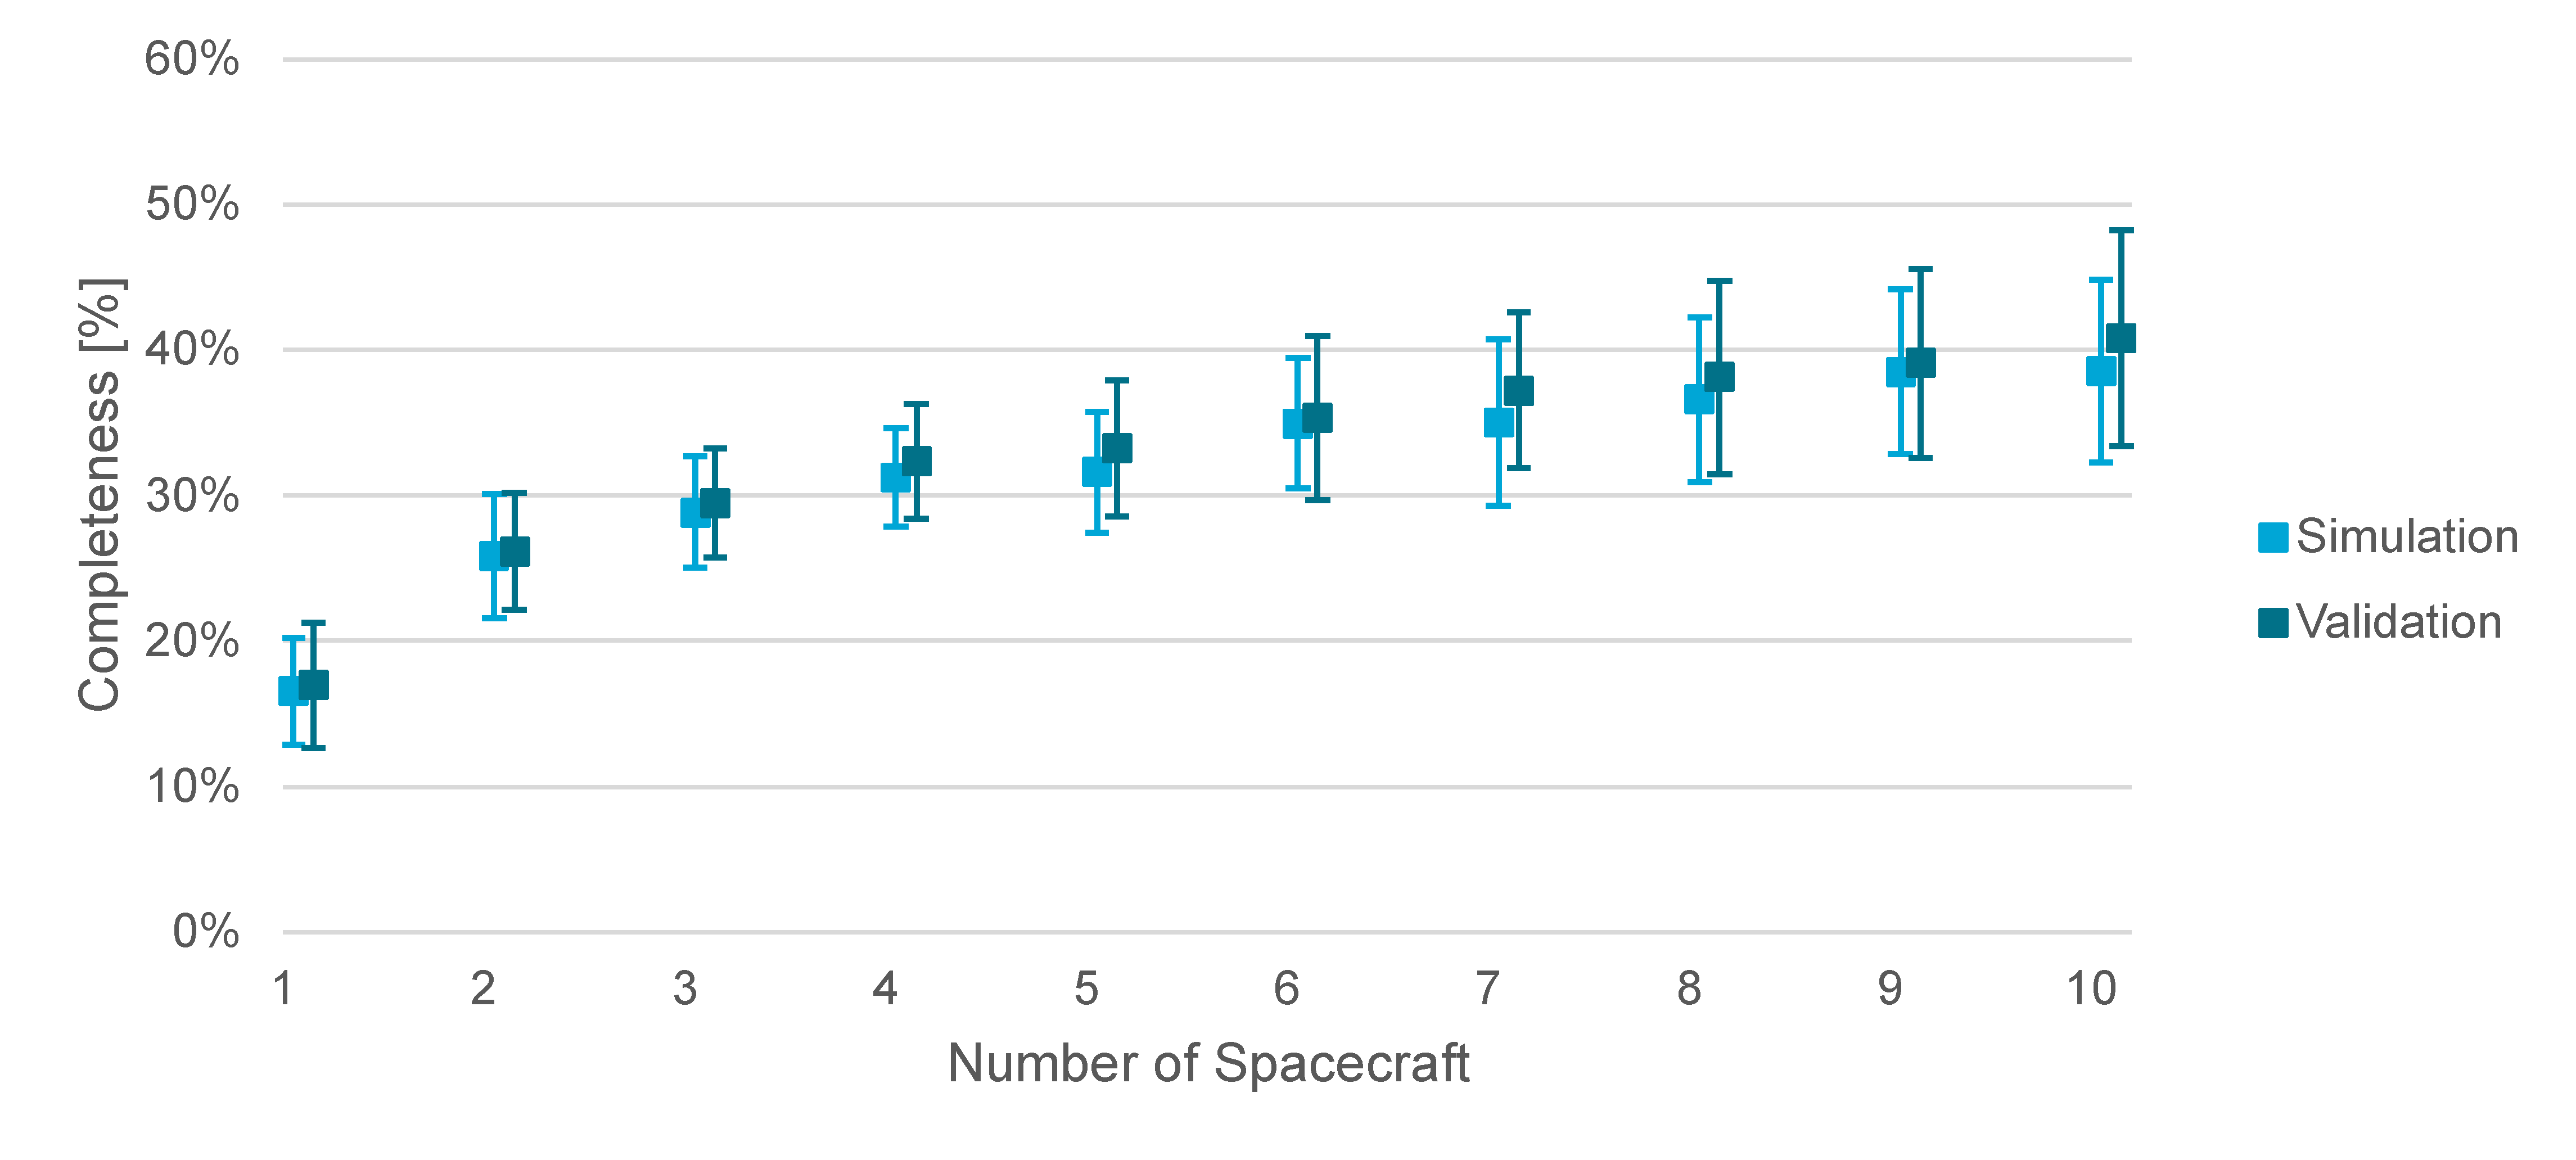
\includegraphics[width=0.7\textwidth]{img/validation_cadence_performance.pdf}
 \caption{Comparison of survey completeness with and without assumptions on survey cadence.}
 \label{fig:validation_cadence_performance}
\end{figure}

\begin{figure}[htbp]
 \centering
 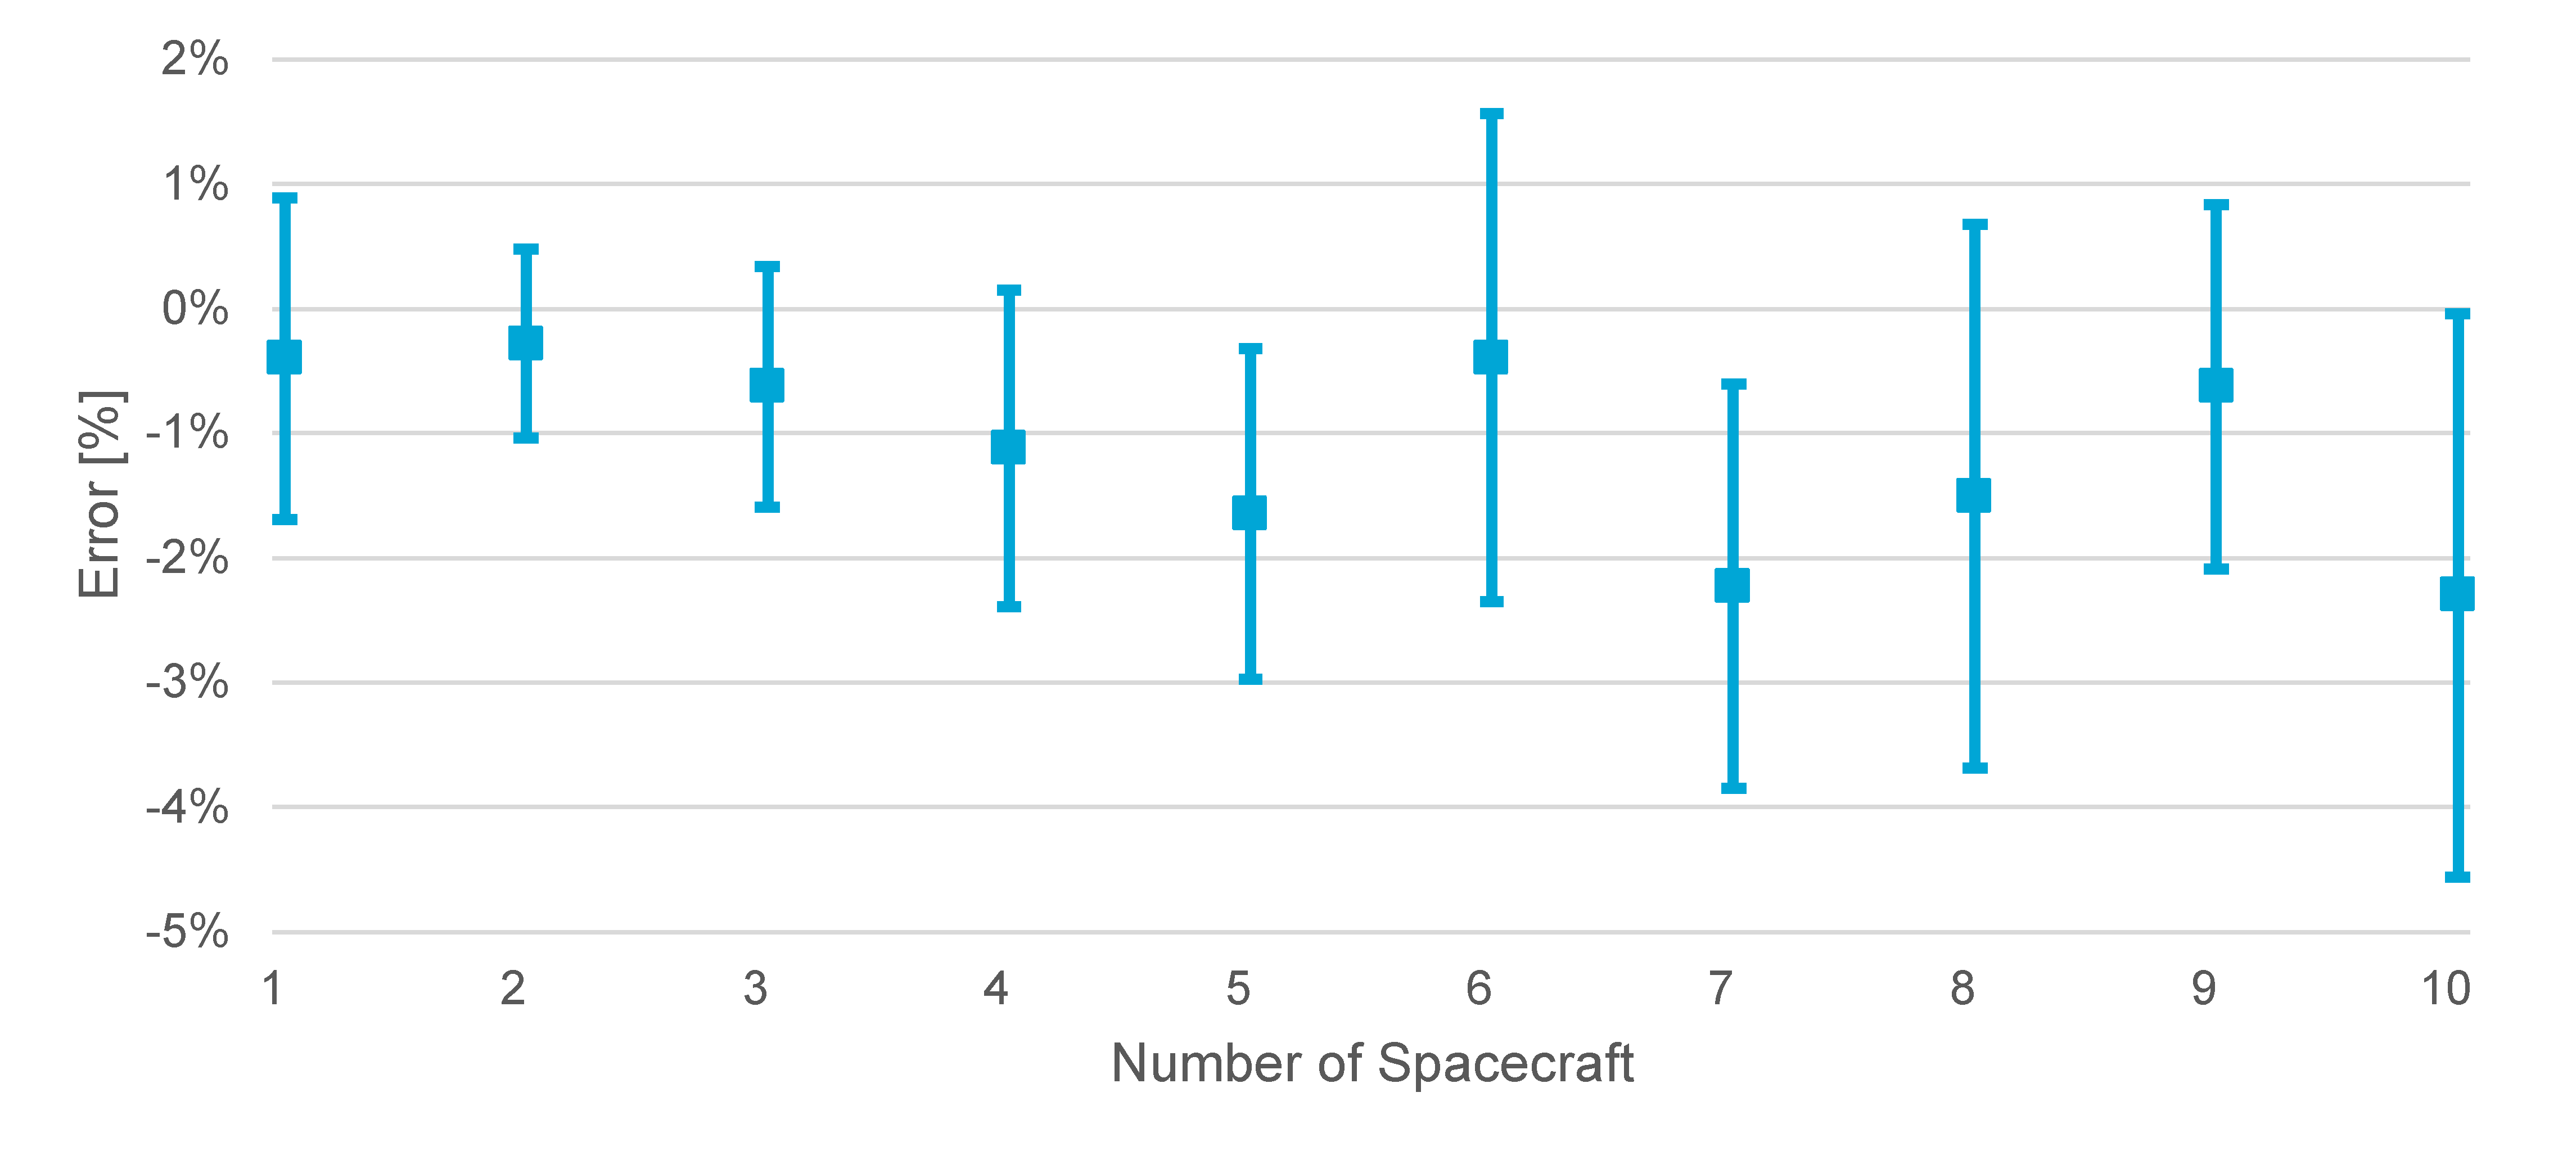
\includegraphics[width=0.7\textwidth]{img/validation_cadence_error.pdf}
 \caption{Error of survey cadence assumption.}
 \label{fig:validation_cadence_error}
\end{figure}

The assumption on cadence implicitly introduces another approximation, however. As the entire sky is imaged at the same time, this also means the spacecraft is imaging towards the Sun. Naturally, aiming a telescope at the Sun is generally ill-advised. Therefore in practice the spacecraft will be limited in how close it can approach the Sun in terms of angular distance. This \textit{maximum solar elongation} $\phi_{max}$ precludes the spacecraft from imaging objects near the Sun. On the other hand, as a smaller area of sky has to be imaged, the survey cadence increases proportionally. Influence of this effect was judged by excluding NEA's below a certain solar elongation from detection. Conversely, the survey cadence was increased by a factor of $\phi_{max}^2 / 4\pi$ to compensate. The results can be seen in \autoref{fig:validation_solar_angle} for $\phi_{max}$ up to $\pi/2$. Even as the number of spacecraft varies, a cut-off point around $\phi_{max} = 1\mathrm{rad}$ is presented. This occurs as most asteroids will be imaged at higher solar elongations; only very few - very large - asteroids can be detected close to the Sun, and at low $\phi_{max}$, the effect on cadence is limited. In addition, these effects have opposite effects on the survey performance, and thus the final impact is negligible.

\begin{figure}[htbp]
 \centering
 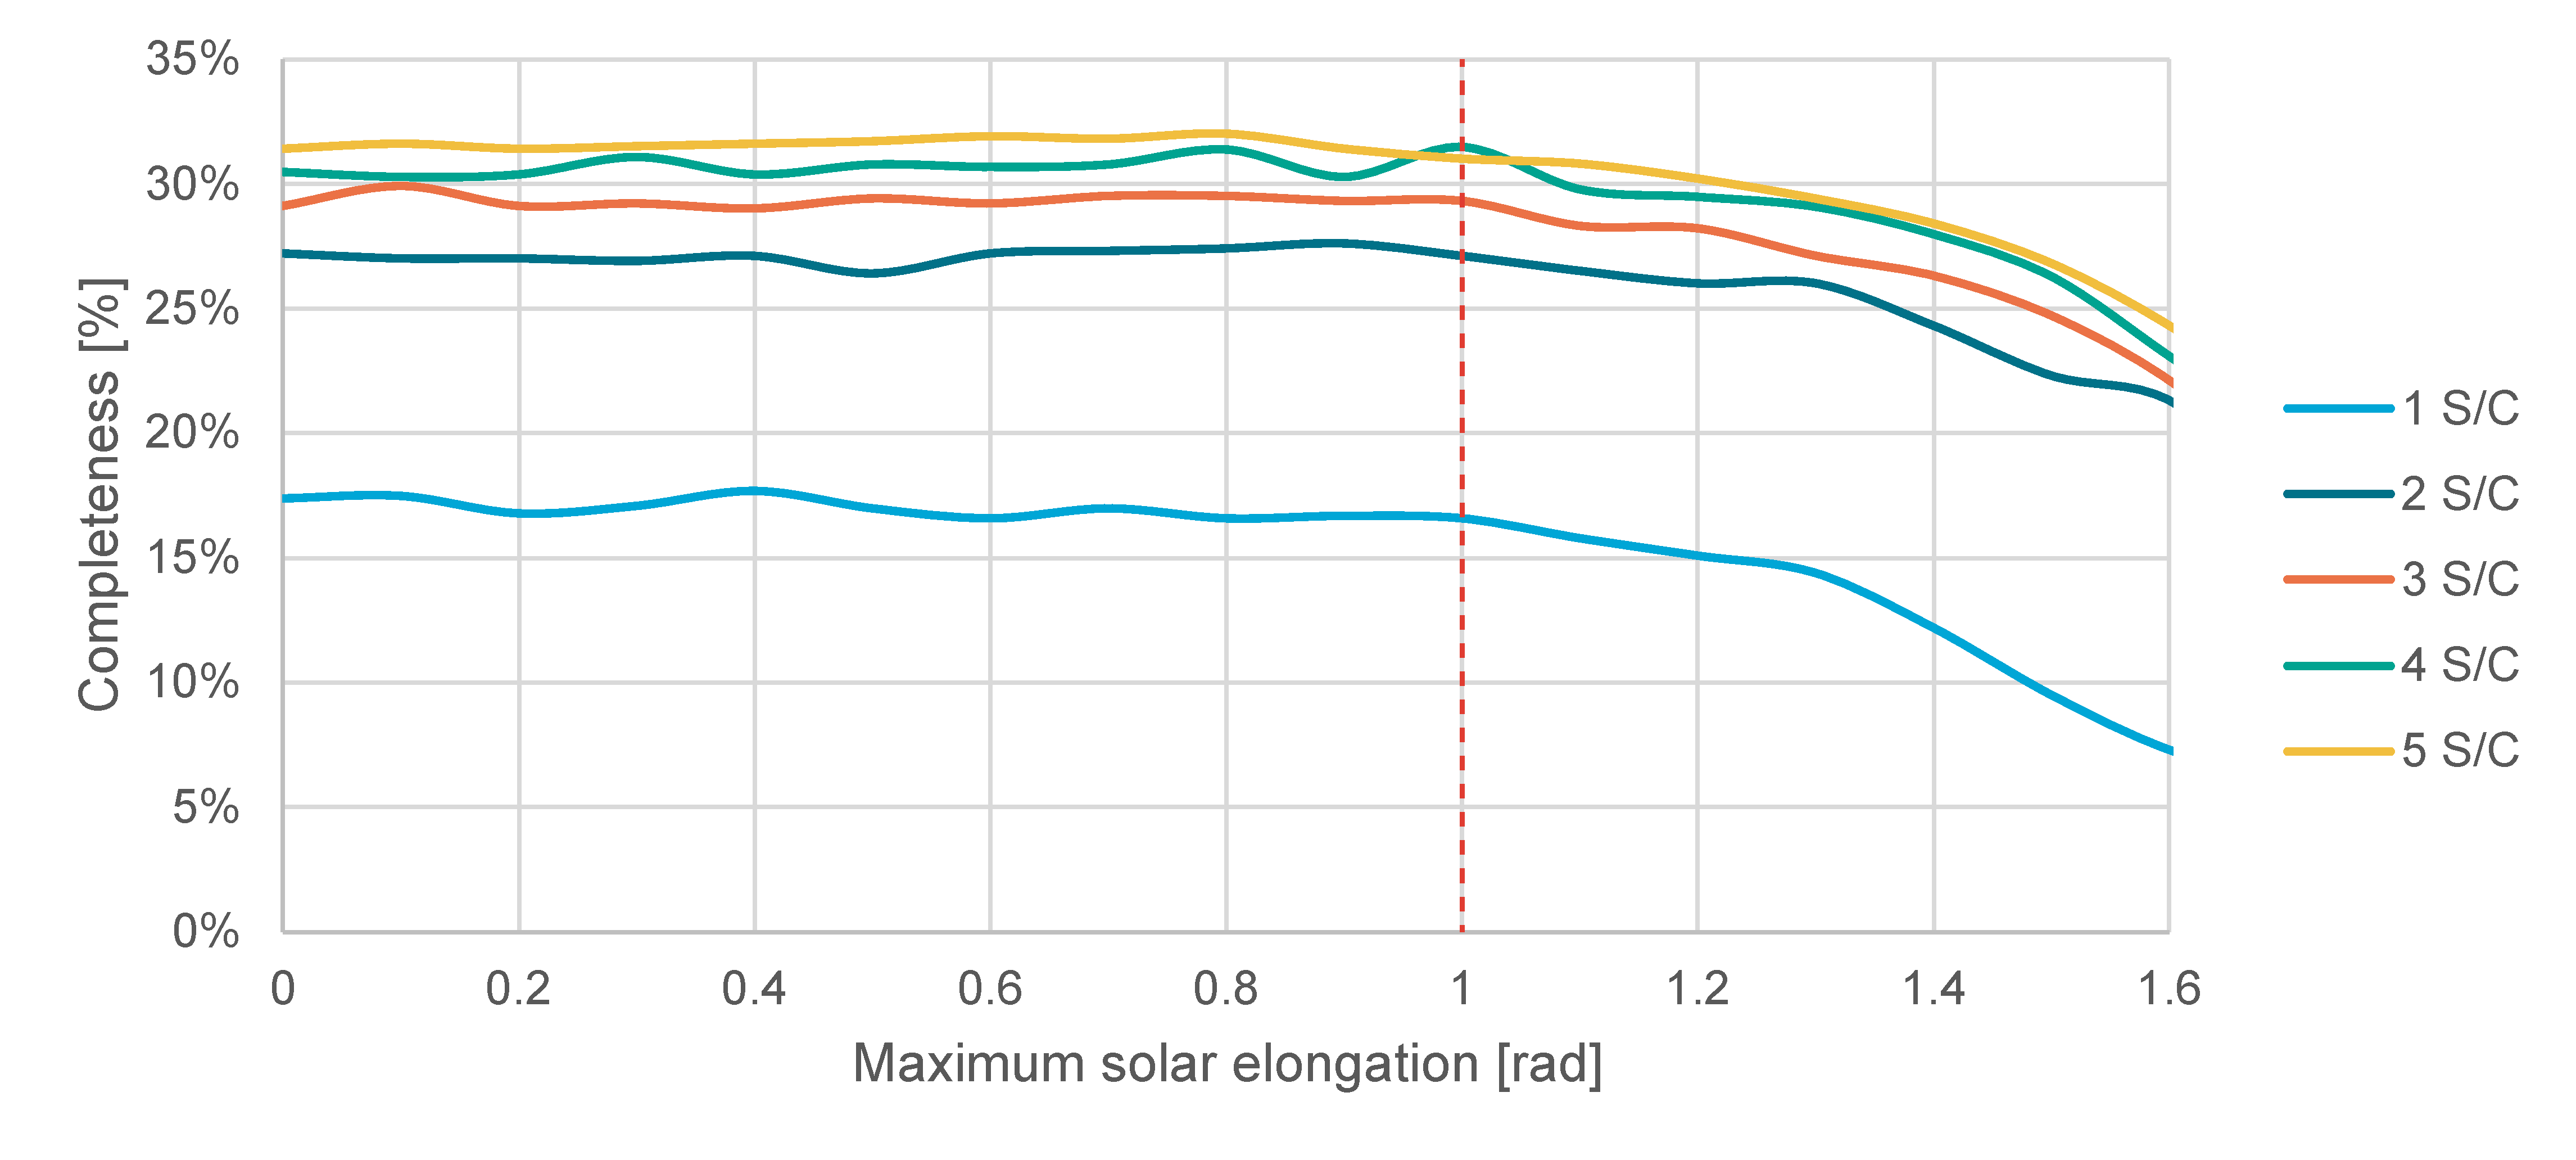
\includegraphics[width=0.7\textwidth]{img/validation_solar_angle.pdf}
 \caption{Expected survey performance as a function of maximum solar elongation.}
 \label{fig:validation_solar_angle}
\end{figure}

A final component of the simulation design has to be adressed, which is the time-dependency of the problem. As the orbits of NEA's are affected by more influences than just the Sun's gravity (see \cite{GranvikPopulation} for a full discussion of this topic), it could be the case that the distribution of asteroids is not entirely homogeneous. In these cases, situations might arise where a time-dependency is introduced into the problem. For example, surveys starting at a later date might show a higher performance than surveys starting earlier due to fluctuations in the asteroids population. Therefore, an analysis was conducted where the survey was simulated offset by a certain period. The results of this simulation can be seen in \autoref{fig:validation_starting_year} for one to four spacecraft. Naturally, some variation is present in the points due to the variance in the simulation. However, there is no significant relationship present between the starting time and the performance of the survey.

\begin{figure}[htbp]
 \centering
 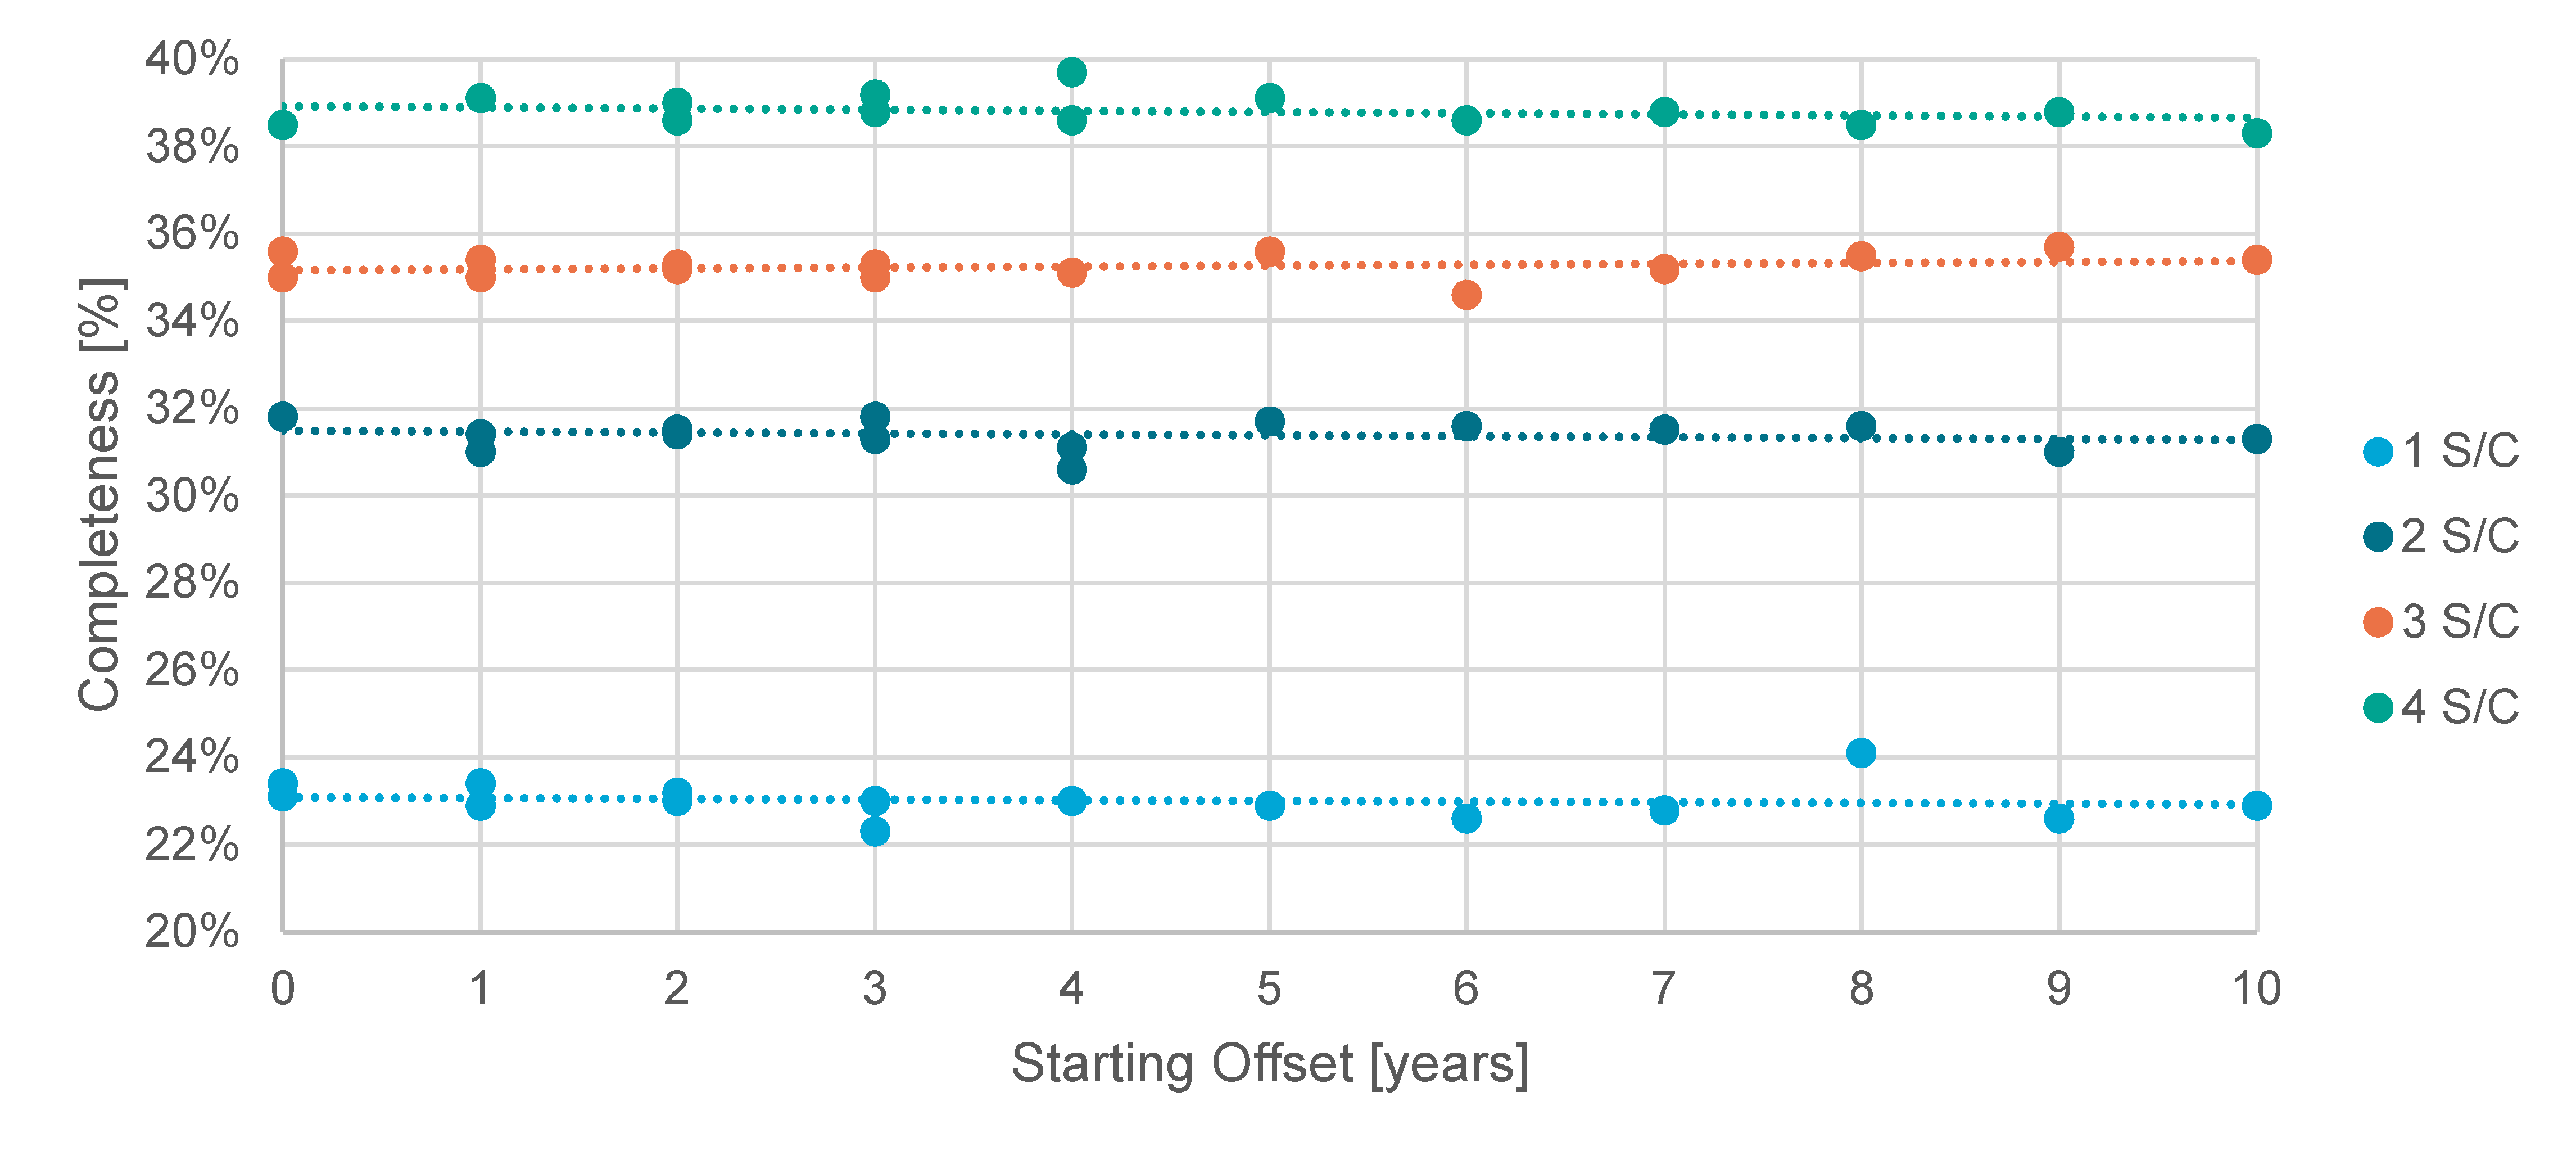
\includegraphics[width=0.7\textwidth]{img/validation_starting_year.pdf}
 \caption{Expected survey performance as a function of the offset in start date.}
 \label{fig:validation_starting_year}
\end{figure}



\section{Expected Performance}
\label{sec:vvperformance}

The last step in the validation procedure was performed to ensure the translation of the simulation predictions to an actual NEA survey. This process was carried out by comparing the results of a simulation to the results of the previously validated survey tool developed by \cite{2017NEOSDT}. It was decided to not compare the survey completeness score, but rather the completeness at various asteroid sizes, as this might help reveal more detailed problems in the simulation. It is noted that a small deviation from the results of \cite{2017NEOSDT} is expected, as some assumptions are made in the simulation in this report, and the used population model for the simulations is slightly different.

\begin{figure}[htbp]
 \centering
 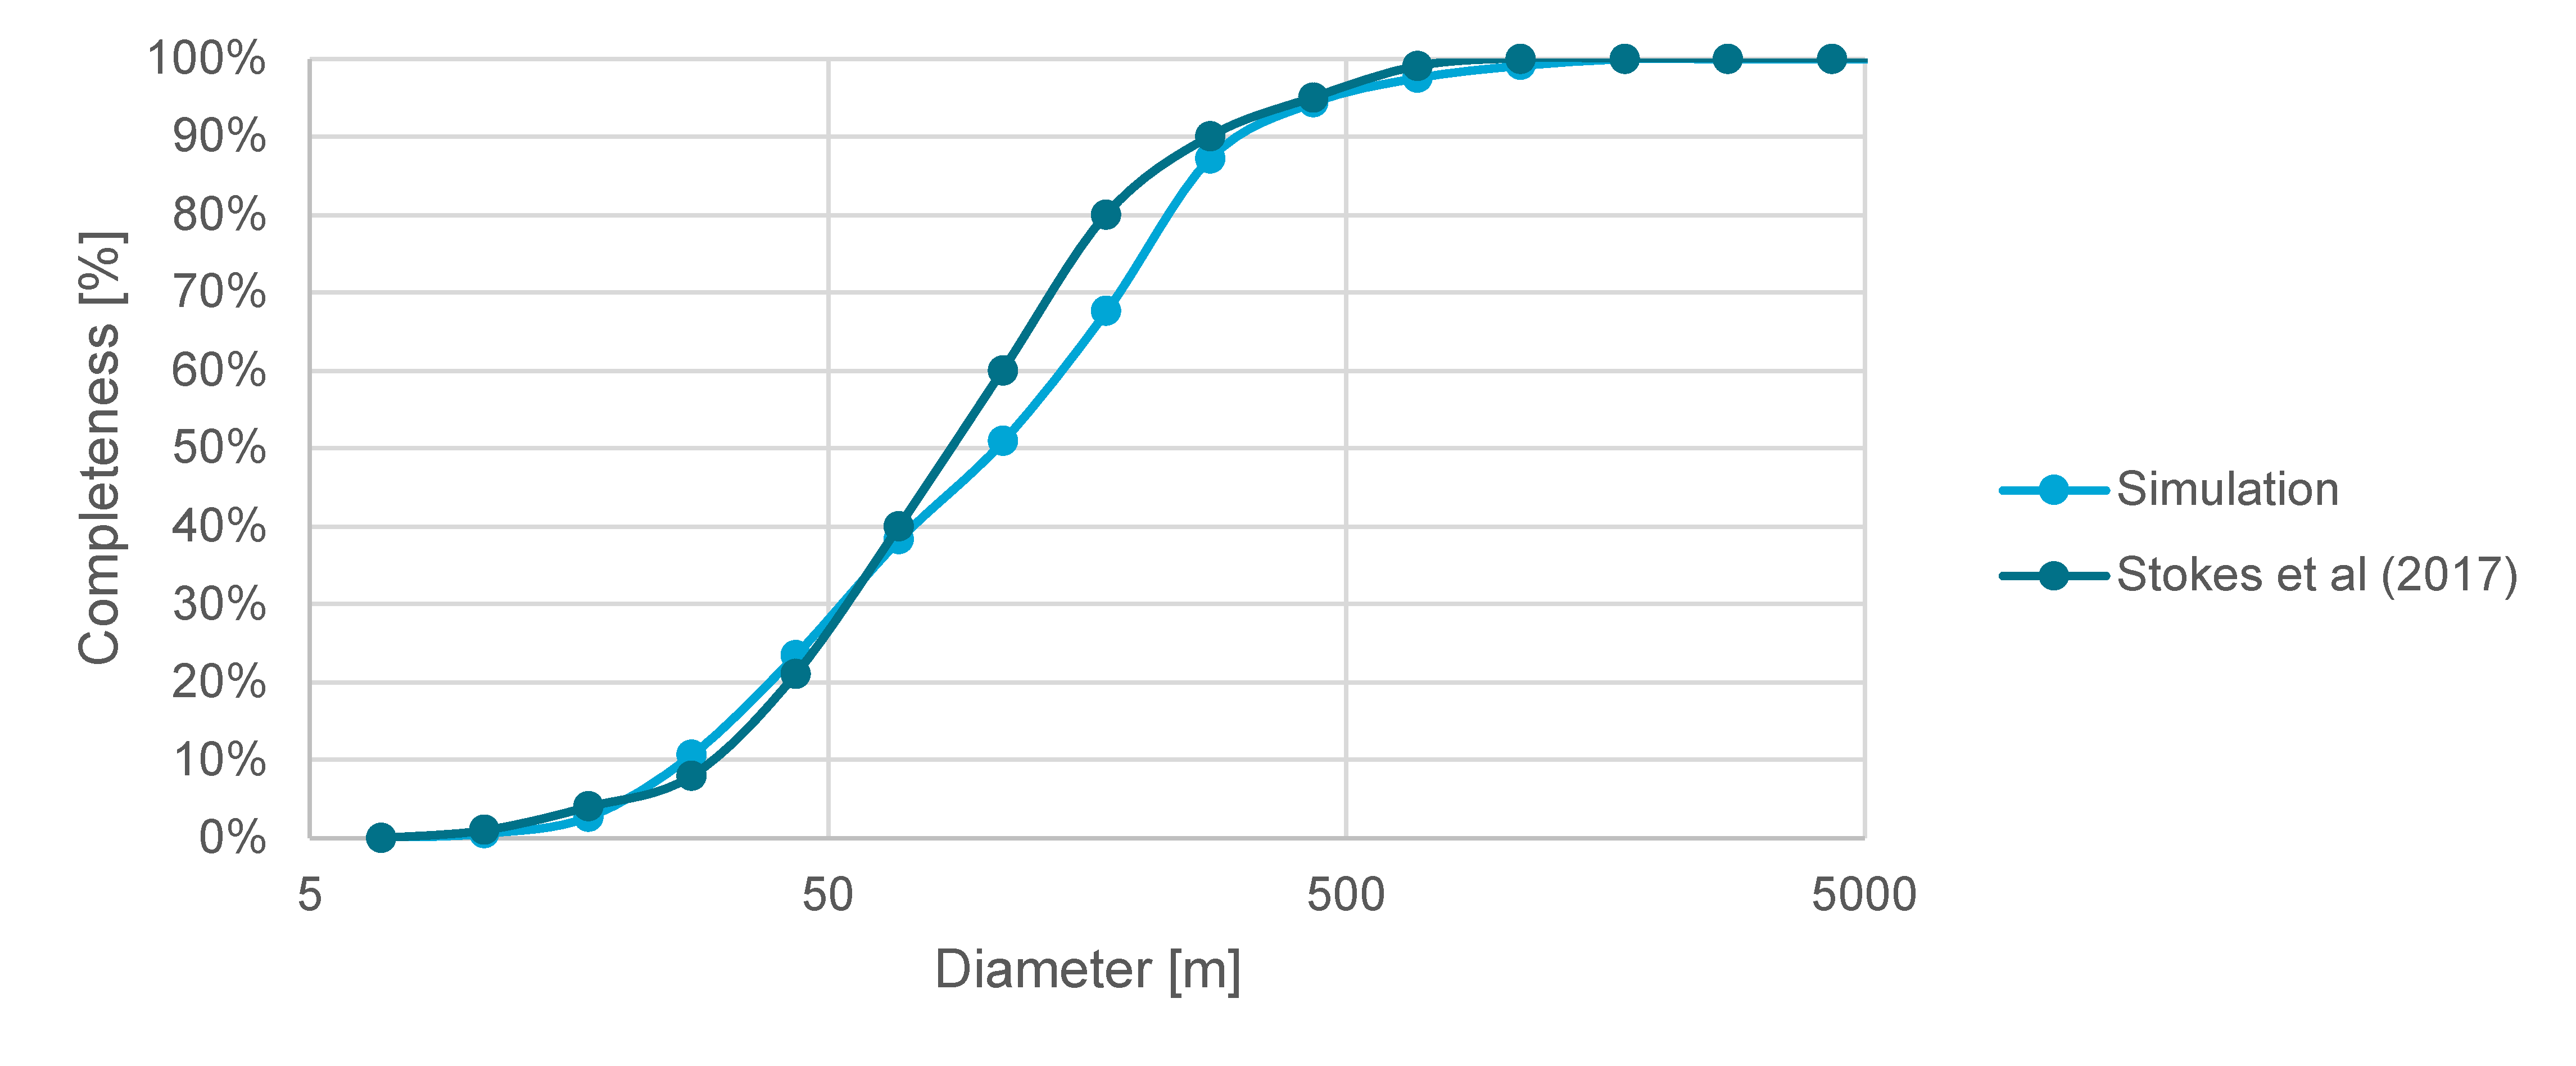
\includegraphics[width=0.7\textwidth]{img/validation_completeness_vis.pdf}
 \caption{Comparison of completeness per absolute magnitude for visual light system, validation data from \cite{2017NEOSDT}.}
 \label{fig:validation_completeness_vis}
\end{figure}


\begin{figure}[htbp]
 \centering
 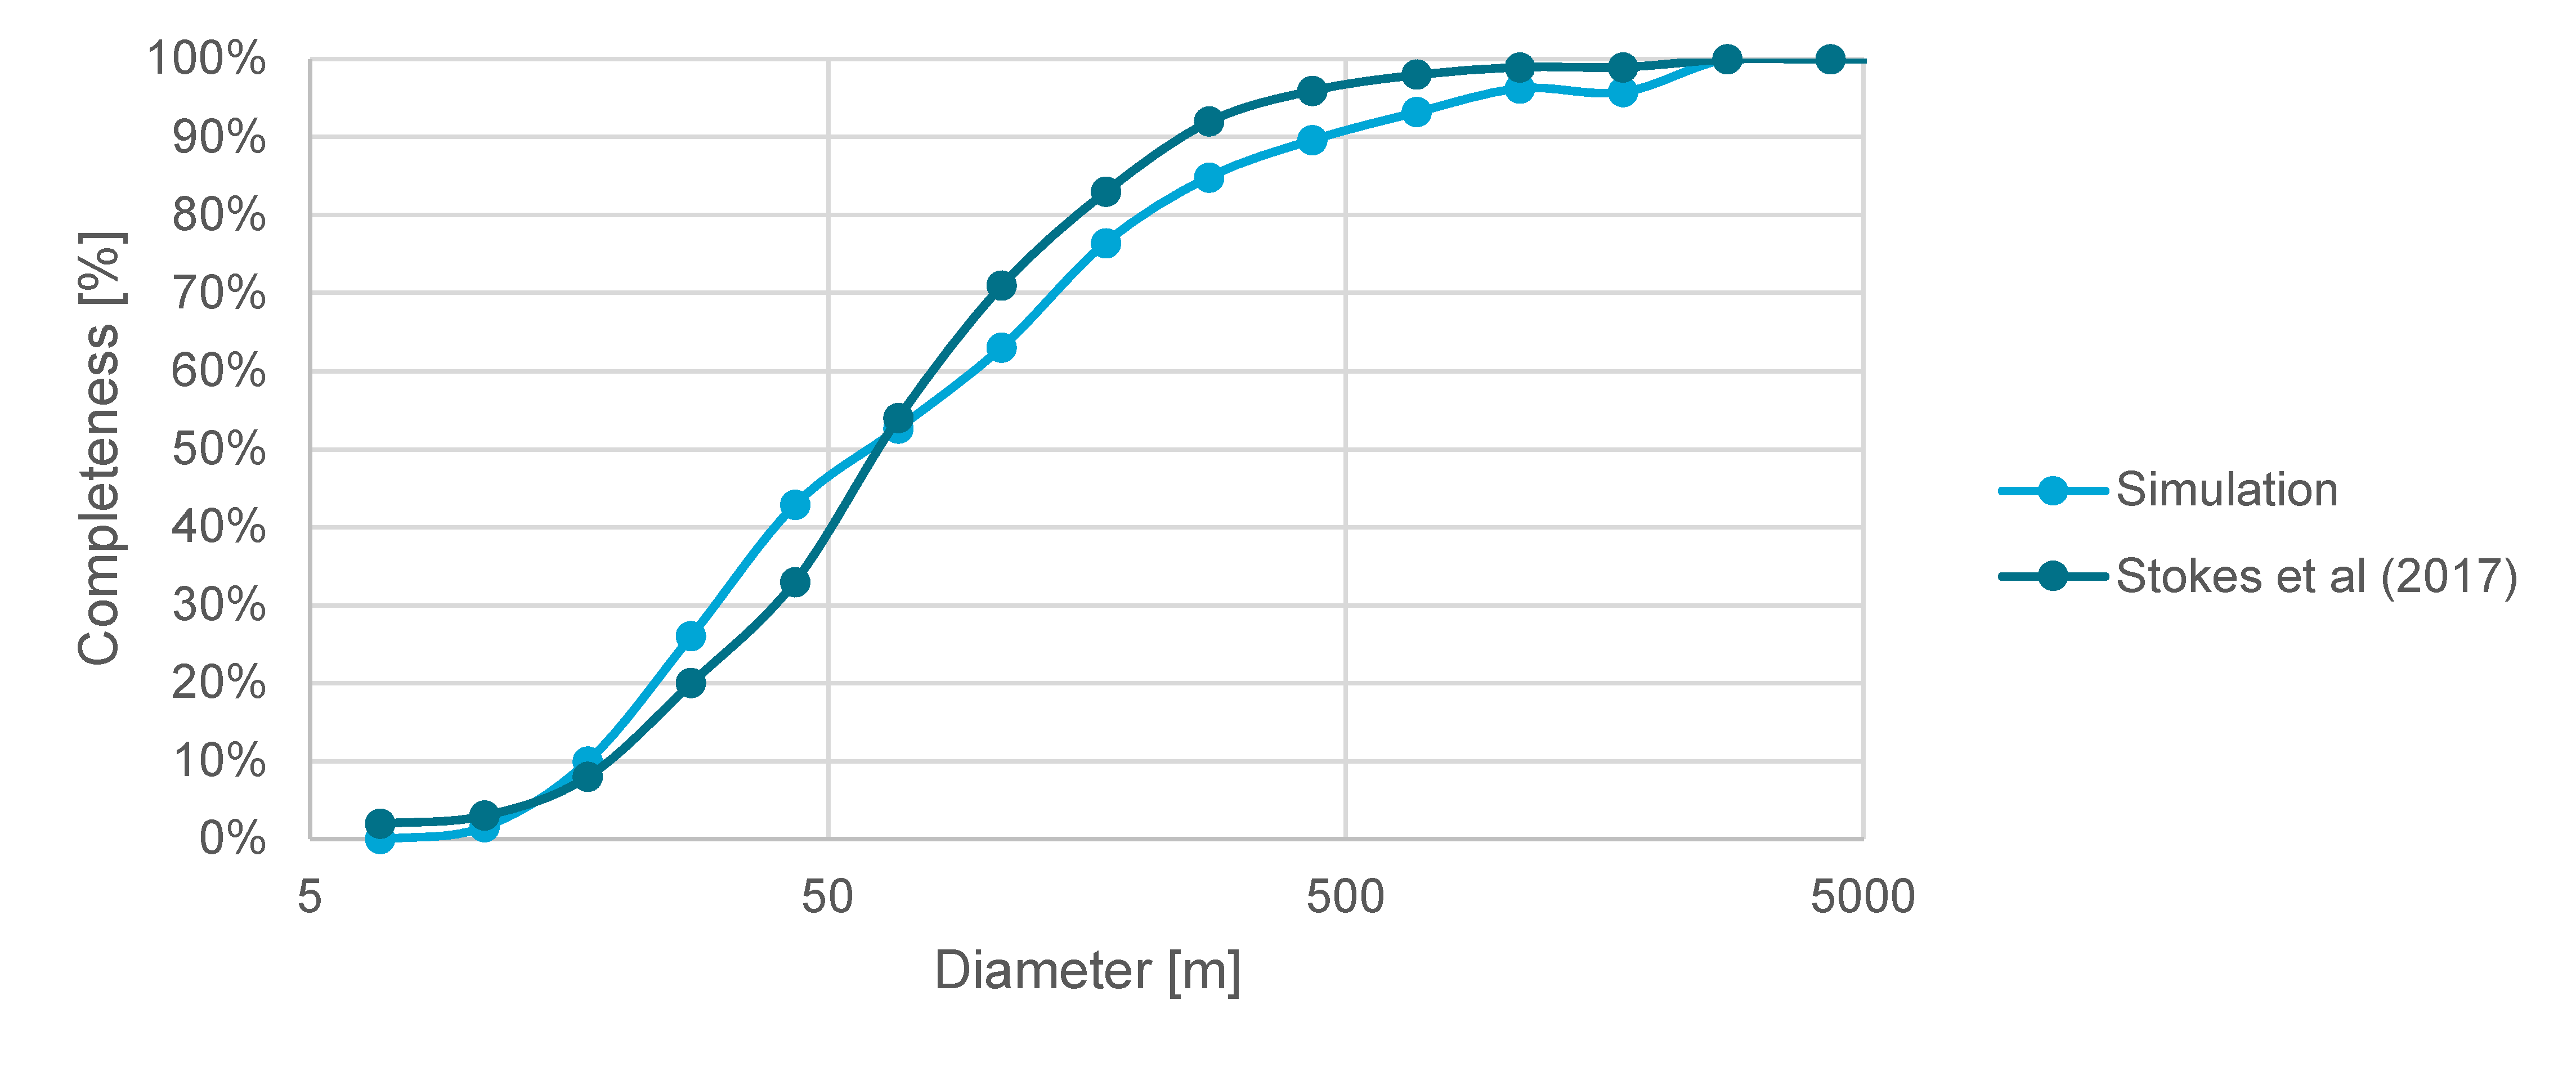
\includegraphics[width=0.7\textwidth]{img/validation_completeness_tir.pdf}
 \caption{Comparison of completeness per absolute magnitude for thermal infrared system, validation data from \cite{2017NEOSDT}.}
 \label{fig:validation_completeness_tir}
\end{figure}

Results of the validation simulations are displayed in \autoref{fig:validation_completeness_vis} and \autoref{fig:validation_completeness_tir} for the visual light and thermal infrared payloads, respectively. Simulations were carried out using the same orbit and payload specifications as used in \cite{2017NEOSDT}. Results appear to be a good approximation. Some variation is however observed: The developed simulation predicts a lower performance for medium-sized asteroids of one to a few hundred meters in diameter, and a slightly higher performance for small-sized asteroids in the range of tens of meters. It is unknown what causes this deviation, although it is speculated that it might occur due to the function used to predict the results of \cite{2017NEOSDT}, as the curve shows almost no variance, whereas some variance would be expected. As the difference is small, and the overall completeness score differs by less than 1\% from the results of \cite{2017NEOSDT}, the simulation tool developed should give results that allow for accurate portrayal of reality, and accurate comparison to other studies and surveys.
